\documentclass{article}

\usepackage{hyperref}
\hypersetup{
    colorlinks=true,
    linkcolor=blue,
    filecolor=magenta,      
    urlcolor=cyan,
}

% for including notebooks
\usepackage{pdfpages}

\usepackage{fancyhdr}
\usepackage{extramarks}
\usepackage{amsmath}
\usepackage{amsthm}
\usepackage{amsfonts}
\usepackage{tikz}
\usepackage{float}
\usepackage[plain]{algorithm}
\usepackage{algpseudocode}
\usepackage{caption}
\usepackage{subcaption}

\usepackage{listings}
\usepackage{color} 
\definecolor{mygreen}{RGB}{28,172,0} 
\definecolor{mylilas}{RGB}{170,55,241}

\lstset{
    basicstyle=\scriptsize\sffamily\color{black},
    frame=single,
    numbers=left,
    showspaces=false,
    showstringspaces=false,
    tabsize=1
}
\lstset{language=Matlab,%
    %basicstyle=\color{red},
    breaklines=true,%
    morekeywords={matlab2tikz},
    keywordstyle=\color{blue},%
    morekeywords=[2]{1}, keywordstyle=[2]{\color{black}},
    identifierstyle=\color{black},%
    stringstyle=\color{mylilas},
    commentstyle=\color{mygreen},%
    showstringspaces=false,%without this there will be a symbol in the places where there is a space
    numbers=left,%
    numberstyle={\tiny \color{black}},% size of the numbers
    numbersep=9pt, % this defines how far the numbers are from the text
    emph=[1]{for,end,break},emphstyle=[1]\color{red}, %some words to emphasise
    %emph=[2]{word1,word2}, emphstyle=[2]{style},    
}

\topmargin=-0.45in
\evensidemargin=0in
\oddsidemargin=0in
\textwidth=6.5in
\textheight=9.0in
\headsep=0.25in


\linespread{1.1}

\pagestyle{fancy}
\fancyhf{}
\lhead{\hmwkAuthorName}
\chead{\hmwkClass: \hmwkTitle}
\rhead{\leftmark}
\lfoot{\lastxmark}
\cfoot{\thepage}

\renewcommand\headrulewidth{0.4pt}
\renewcommand\footrulewidth{0.4pt}

\setlength\parindent{0pt}

\newcommand{\hmwkTitle}{Assignment \ 1}
\newcommand{\hmwkDueDate}{March 10, 2020}
\newcommand{\hmwkClass}{Introduction to AI}
\newcommand{\hmwkClassInstructor}{Dr. Joseph Brown}
\newcommand{\hmwkAuthorName}{\textbf{Artem Bakhanov (B18-03)}}

%
% Title Page
%

\title{
    \vspace{2in}
    \textmd{\textbf{\hmwkClass:\ \hmwkTitle}}\\
    \normalsize\vspace{0.1in}\small{Due\ on\ \hmwkDueDate\ at 11:59pm}\\
    \vspace{0.1in}\large{\textit{\hmwkClassInstructor\ }}
    \vspace{3in}
}

\author{\hmwkAuthorName}
\date{}

\begin{document}

\maketitle

\pagebreak

\tableofcontents

\pagebreak

\section{Introduction}
\subsection{General information}
    The assignment is solved by me, Artem Bakhanov, a student of Innopolis University. If you have any question regarding any part of this document and other provided materials, you can contact me via email: \href{mailto:a.bahanov@innopolis.university}{a.bahanov@innopolis.university}.\\
    In this assignment I used SWI Prolog of version 8.0.3-1. It can be easily downloaded from the official \href{https://www.swi-prolog.org/download/stable}{website}. I highly recommend you to use \href{https://marketplace.visualstudio.com/items?itemName=arthurwang.vsc-prolog}{VCS-Prolog} extension for Visual Studio Code. 
\subsection{Tests}
All the tests are created by me (except for the first one, which was taken from the assignment text). You can find them in the directory called "tests". They are simple prolog files with predefined predicates. Note that I use predicates \texttt{player(+Position)}, \texttt{orc(+Position)}, and \texttt{touchdown(+Position)} for defining players', orcs' and touchdowns positions respectively, where \texttt{Position} is a position predicate \texttt{p(X, Y)} with X and Y coordinates. X-axis is a horizontal axis directed to the right, Y-axis is a vertical one directed upward (please see figures ~\ref{fig:test1} and ~\ref{fig:test2}). 
\lstinputlisting[caption=Test 1={lst:listing1}, language=Prolog]{tests/input1.pro}

\begin{figure}[ht]
   	 \centering
     \begin{subfigure}[b]{0.45\textwidth}
         \centering
         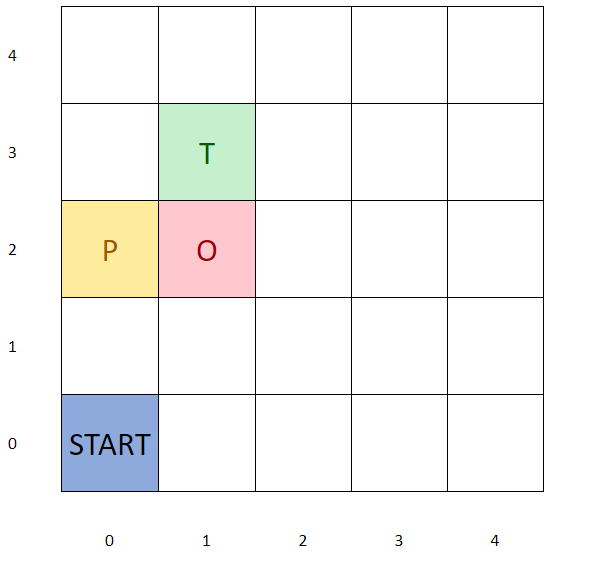
\includegraphics[width=\textwidth]{images/image1.png}
         \caption{Test 1}
         \label{fig:test1}
     \end{subfigure}
     \hfill
     \begin{subfigure}[b]{0.45\textwidth}
         \centering
         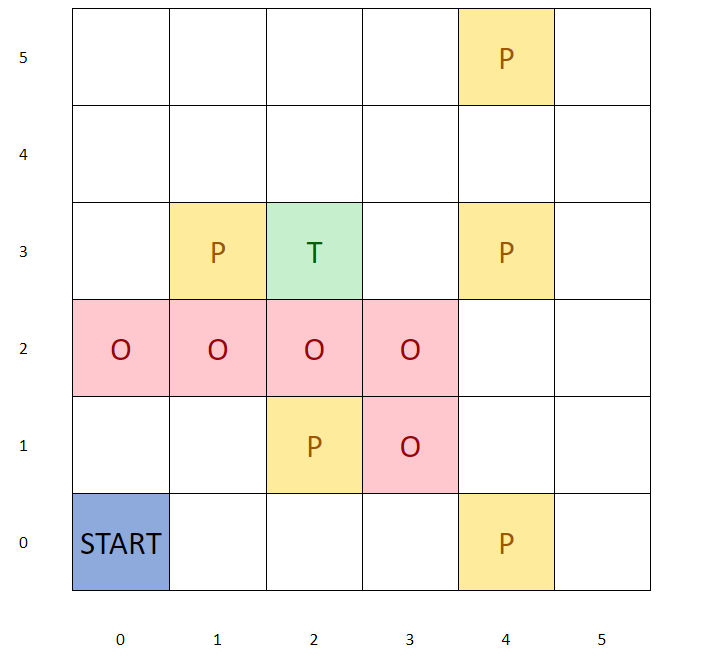
\includegraphics[width=\textwidth]{images/image2.png}
         \caption{Test 2}
         \label{fig:test2}
     \end{subfigure}
     \caption{Examples of tests}
\end{figure}
Here and throughout I mark players (humans) as P (yellow), orcs as O (red), touchdowns as T (green). The start is always situated at $(0, 0)$. By the conventions, player at the start cell is implicitly specified in the input files.

\subsection{Running the code}
To run the program you need to execute \url{main.pl} file and run the following query: \texttt{?- start(Number).} where \texttt{Number} is 0, 1, or 2, which stands for Backtracking Search, Random Search, and new Search, respectively. The result will be printed to the standard output of the interpreter. 

\section{Algorithms}
\subsection{Backtracking Algorithm}
I implemented the backtracking algorithm using the Prolog Tree. The algorithm finds the first solution and returns it. There is no randomness in the implementation, so the algorithm tries to traverse the map spirally. In the backtracking search, the algorithm tries all the possible movements, including ball passes (if it was not performed earlier).\\
There are several assumptions I made during coding the algorithm.
\begin{enumerate}
	\item There is no need to return to a cell where the ball was before (i.e. duplicated move).
	\item Since the ball cannot return to any old position, there is no need to move players. All the positions are static predicates.
	\item There is no need to pass a ball over a cell where it was before. For example, if player 1 passes a ball from $(2, 1)$ to player 1 located in $(2, 5)$ after player 1 came to $(2, 1)$ from $(2, 3)$, then there is no reason no make such a pass because it could be made earlier.
	\item Handoff is a move but with 0 cost.
	\item The start position of the ball is not saved while performing the backtracking search since the ball cannot enter $(0, 0)$ twice and exit from there because of forbidden duplicated moves.
\end{enumerate}
A very important metric of the algorithm is its time complexity. Since the algorithm is exponentially complex its execution time can be high on the big maps (e.g. 10*10). On big maps with "unusual" field configuration, the algorithm needs a lot of time. For instance, the algorithm does not work on test 7 faster than 5 minutes (I did not run the algorithm for a longer time). Note that the problem with the test is just a \texttt{move} predicate order. The algorithm goes in this order: it tries to pass the ball from upward clockwise, then it tries to move a player from upward clockwise.

\subsection{Random Search}
The random search is very similar to the backtracking search except for the implementation of \texttt{move} predicate. I create new predicate \texttt{select\_random\_move(...)}, which literally selects only one move at a time (I used cut to avoid backtracking behaviour). The second difference is that the random search performs exactly 100 moves in one round. I simulate 100000 rounds and select the best solution. I used the same assumptions as I used for backtracking search.\\
The time complexity of the algorithm is always constant since the algorithm performs the same amount of work for any input (100 moves for each round). 

\subsection{BFS}
The third algorithm I implemented was actually an experiment that I liked and want to present. I implemented recursive BFS using prolog tree. It is easy to implement queue in Prolog (just a list with).

\section{Advanced Team}
\subsection{Backtracking Algorithm}
There is no improvement of the algorithm since it works like trial and error methods. It \textbf{tries}, if no success, it rolls back and try another way. 
\subsection{Random Search}
Random search will not get any improvement too, since it takes purely random moves, which does not depend on the environment.
\subsection{Improved Backtracking Search}
The situation is the same for this search as for the backtracking search. Since I do not use any heuristic function, extended visibility does not help at all.
\subsection{Conclusion}
There is no difference when it comes to distance of visible objects, therefore there is no improvement on the algorithms' time complexity. This methods will not make unsolvable map solvable and vice versa.
It is important to mention that for some algorithms extended visibility might help to improve its performance. The very obvious examples of such algorithms are A* (heuristic function) and Tabu (Tabu lists can be created without visiting certain cells) searches.

\section{Hard Maps}
There are different hard or impossible maps for different algorithms. 
Let us talk about backtracking algorithm.
\subsection{Backtracking Algorithm}
In case of this algorithm, it is hard to find a solution when the map forces player to start freely move from the center of the map. Example of such a map is input 7 that is shown on the picture below. As you can see, we can treat the start of the field at $(4, 0)$ where the algorithm literally starts from. Since the order of movements are from up to left (clockwise), the algorithm will stuck in the $X = [5, 10]$ area before it goes to the left.
\begin{figure}[ht]
        \centering
        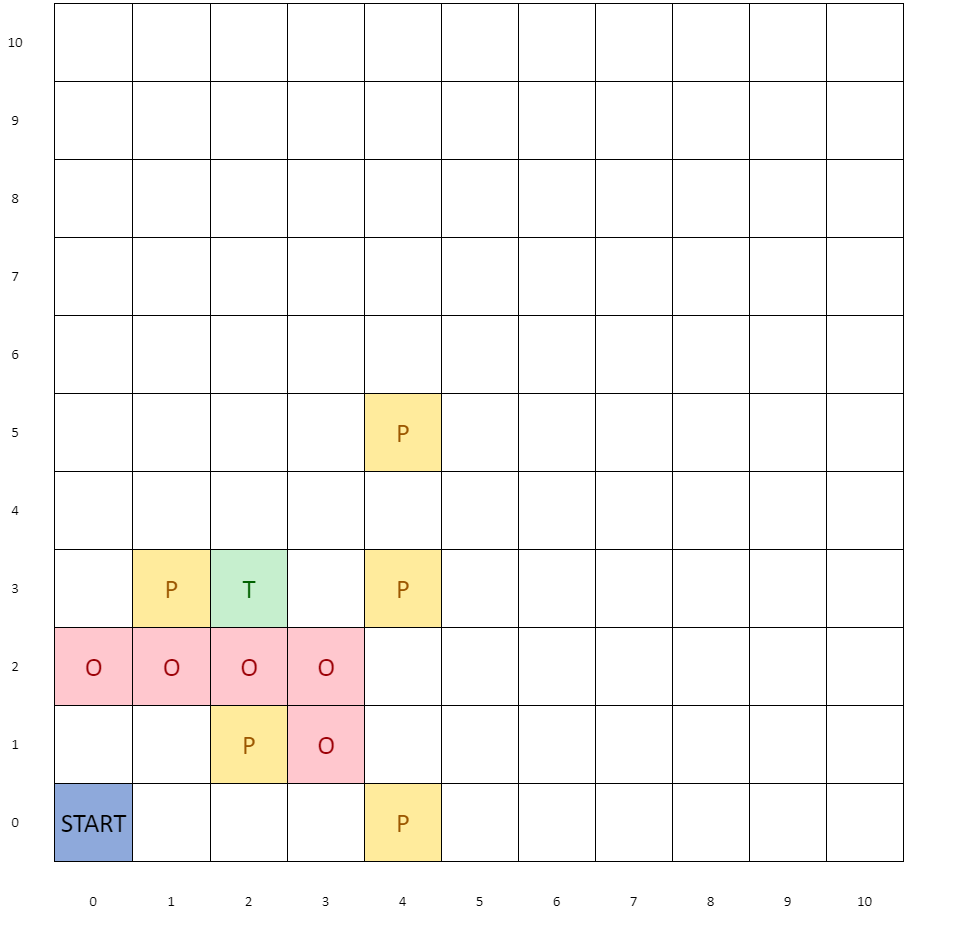
\includegraphics[width=0.75\textwidth]{images/image3.png}
        \caption{Test 7 - impossible one}
        \label{fig:test7}
\end{figure}
\end{document}
